\documentclass[10pt]{article}

\usepackage[a4paper,left=0.5cm,right=0.5cm,top=0.5cm,bottom=0.5cm]{geometry}
\usepackage{multicol}
\usepackage{graphicx}
\usepackage{calc}
\usepackage{enumitem}
\usepackage[usenames,dvipsnames]{xcolor}
\usepackage{fancybox}
\usepackage{tabularx}
\usepackage{booktabs}

\usepackage{fontspec}
\setmainfont{equity}[
  % Files
  Path      = \string~/s/fonts/equity/ ,
  Extension = .otf ,
  % Fonts
  UprightFont     = Equity Text A Regular ,
  UprightFeatures = { SmallCapsFont = Equity Caps A Regular } ,
  BoldFont        = Equity Text A Bold ,
  BoldFeatures    = { SmallCapsFont = Equity Caps A Bold } ,
  ItalicFont      = Equity Text A Italic ,
  BoldItalicFont  = Equity Text A Bold Italic ,
  % Features
  Numbers = OldStyle ]

\usepackage{parskip}
\setlength{\parskip}{\medskipamount}

\newcommand\locationcolour{Mahogany}
\newcommand\npccolour{CornflowerBlue}
\newcommand\headingcolour{\locationcolour}

\usepackage{tcolorbox}
\usepackage{xpatch}
\xpatchcmd{\section}{\normalfont\Large\bfseries}{\sectionbox}{}{\PatchFailed}
\newcommand*{\sectionbox}[1]{%
\begin{tcolorbox}[
  colback=\headingcolour,
  colframe=\headingcolour,
  coltext=white,
  height=2\baselineskip,
  valign=center,
  sharp corners
]
  \textsc{\large #1}
\end{tcolorbox}
}

\pagestyle{empty}
\nonfrenchspacing

\newcommand{\keyword}[1]{\textsc{\textbf{#1}}}
\newcommand{\location}[1]{\keyword{\color{\locationcolour}#1}}
\newcommand{\npc}[1]{\keyword{\color{\npccolour}#1}}

\title{1406, The Golden Wood}

\begin{document}

\begin{center}
{\Huge 1406}

{\large \textsc{The Golden Wood}}

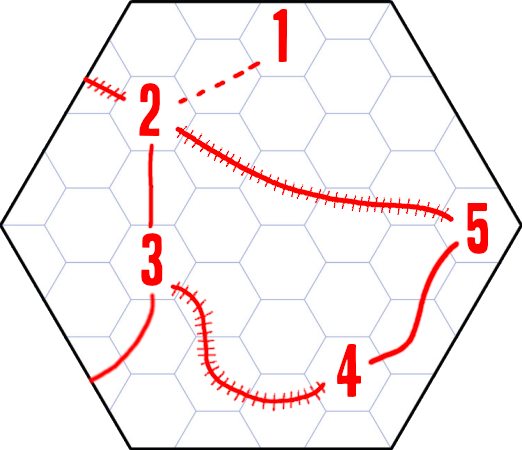
\includegraphics[scale=0.5]{hexmap}

\emph{The party quest for \keyword{knobbled mandrake} to save their
companion, but it can only be found in \location{The Mandrake
  Patch}\\or in the fairy realm of \location{Whyforth} which lies
beyond the \keyword{yellow doors}}.

\keyword{Random Encounters:}
1--2, \textbf{1d4} elf knights;
3--4, \npc{Majorus} or \npc{Braithlynne};
5--6, Aldweald encounter.
\end{center}

\begin{multicols*}{2}
\section{The Mandrake Patch}

%% Size: 1 (a stump, a large puddle)

A \keyword{squirming patch of earth} with a strong scent of plums.
Glowing head-sized \keyword{fungal orbs} illuminate everything with a
golden light.

A \keyword{hidden animal trail} heads south-west to \location{Azeria's
  Court}.

Digging in the \keyword{squirming earth} yields \textbf{1d4} portions
of \keyword{knobbled mandrake}.

The \keyword{fungal orbs} glow for 24 hours when plucked.

A \keyword{yellow door} lies between the roots of an old tree.

\section{Azeria's Court}

%% Size: 3 (a house, a large ring of stones)

A house-sized clearing.  A weathered \keyword{mosaic} visible beneath
the grass.  \npc{Azeria}, the Royal Fox, holds court.  Glowing
head-sized \keyword{fungal orbs} illuminate everything with a golden
light.

A \keyword{hidden animal trail} heads north-east to \location{The
  Mandrake Patch}.

A \keyword{boggy trail} heads north-west to \location{hex 1306}.

A \keyword{well-trodden deer path} heads south to \location{The
  Obelisk}.

A \keyword{thin nettle-encrusted trail through the bog} heads
south-east to \location{The Abandoned Camp}.

The \keyword{mosaic} depicts the gardens of \location{Whyforth} and
the seven \keyword{yellow doors}.

The \keyword{fungal orbs} glow for 24 hours when plucked.

A \keyword{yellow door} is inside the mosaic, looking just like a part
of the picture unless detected.

\section{The Obelisk}

%% Size: 5 (a hillside, a cow pasture)

A rough-hewn dolomite \keyword{obelisk}, which hums faintly.
\npc{Majorus} can often be found here studying the arcane residue.

A \keyword{well-trodden deer path} heads north to \location{Azeria's
  Court}.

A \keyword{path of unevenly-placed stones across the bog} heads
south-east to \location{The Drune Cottage}.

A \keyword{well-trodden deer path} heads south to \location{hex 1307}.

Touching the \keyword{obelisk} teleports the character to
\location{hex 0703}, where there is an identical obelisk which can
teleport them back.

A \keyword{yellow door} lies rippling in a puddle's reflection.

\section{The Drune Cottage}

%% Size: 6 (a ruined abbey, an acre of trees)

A lonely thatched-roof stone cottage with two large gardens and a pen
with a dozen chickens, three goats, and a cow.  A family of three
Drune live here.

A \keyword{path of unevenly-placed stones across the bog} heads
south-west to \location{The Obelisk}.

A \keyword{slightly overgrown path} heads north-east to \location{The
  Abandoned Camp}.

The \keyword{inhabitants} are \npc{Majorus}, Drune Cottager;
\npc{Estembra}, Drunewife; and \npc{Braithlynne}, Drune Braithmaid.

A \keyword{yellow door} is buried and sealed by Drunic magic.

\section{The Abandoned Camp}

%% Size: 2 (a small grove, a campsite)

An abandoned campsite strewn with rubbish and a few decaying tents.
Once the home of some ne'er-do-wells who preyed upon travellers of the
horse-eye road to the south and south-west.

A \keyword{thin nettle-encrusted trail through the bog} heads
north-west to \location{Azeria's Court}.

A \keyword{slightly overgrown path} heads south-west to \location{The
  Drune Cottage}.

A \keyword{yellow door} stands, tall and wooden and out of place,
inside one of the tents.

\section*{The Fairy Realm of Whyforth}

As in the \emph{Dolmenwood Campaign Book}, except that
\keyword{knobbled mandrake} (along with other rare plants) can be
found in the gardens by the doors.

\keyword{Elf Knights} quickly arrive to chase off any uninvited
guests.

\renewcommand\headingcolour{\npccolour}

\section*{Azeria, Royal Fox}

\emph{Into the Wyrd and Wild} page 112.

A beautiful fox bedecked in fine jewellery, in service to Yorghan.
Has diplomatic ties to half the fairy nobility of Dolmenwood, and
secretly to House Brackenwold too.  Has negotiated immunity to time
and sickness with the primal deities of such: will never disclose what
she gave up in return.

\begin{description}[leftmargin=!,labelwidth=\widthof{\bfseries Demeanour}]
\item[Demeanour] Regal, proud, intelligent, braggadocious.  Intrigued
  by the presence of unfamiliar mortals.
\item[Speech] Eloquent, well-enunciated.  Woldish, Old Woldish,
  Sylvan, High Elfish.
\item[Wants] Stories.
\item[Knows] About the powerful factions of the wood and their aims.
  The secret of the \keyword{yellow doors}.  Where to find
  \keyword{knobbled mandrake}.
\item[Spells] \emph{dancing lights}, \emph{false aura},
  \emph{nondetection}.
\item[Treasure] coronet worth 200gp; earrings worth 4$\times$50gp;
  gem-encrusted torcs worth 2$\times$100gp; bracelet worth 50gp.
\end{description}

\section*{Majorus, Drune Cottager}

\emph{Dolmenwood Monster Book} page 36.

A tall thin man wrapped in a stained travelling cloak, carries a
gnarled wooden staff and wears a featureless clay mask.  Spends his
days studying the magic of \location{The Obelisk}.

\begin{description}[leftmargin=!,labelwidth=\widthof{\bfseries Demeanour}]
\item[Demeanour] Unfriendly, hostile, intrigued by arcane secrets.
  Hard of hearing.
\item[Speech] Harsh and brief, just enough words to get his point
  across and no more.  Woldish, Drunic.
\item[Wants] Non-Drune to leave the wilds, to return to the roads and
  towns of civilisation and not bother his work.
\item[Knows] About \npc{Azeria}, the Royal Fox, and that she has
  dealings with fairy.
\item[Sigil] \emph{fear}, save vs spells or flee (1 turn).
\item[Spells] \emph{charm person}, \emph{darkness}, \emph{sleep},
  \emph{hold person}.
\end{description}

\section*{Estembra, Drunewife}

\emph{Dolmenwood Monster Book} page 37.

A beaming and buxom woman, dressed in dyed skins and with a necklace
of squirrel skulls.  Spends her days keeping house, gardening, and
tending to the animals.

\begin{description}[leftmargin=!,labelwidth=\widthof{\bfseries Demeanour}]
\item[Demeanour] Friendly and welcoming, grandmotherly.  But will
  instantly turn hostile to non-Drune she deems a threat.
\item[Speech] Overly familiar, even with complete strangers.  Calls
  people ``dearie'' a lot.  Speaks to animals as if they understand
  (do they?).  Woldish, Drunic.
\item[Wants] To live a quiet life in her cottage with her family.  For
  \npc{Braithlynne} to become a witch.
\item[Knows] The finding and usage of herbs, including the location of
  \location{The Mandrake Patch}.
\item[Kilnling] \emph{guardian}, placed beside the path to
  \location{the Drune Cottage}, save vs spells or be turned to clay,
  shrieks and shatters if an intruder passes their save.
\end{description}

\section*{Braithlynne, Drune Braithmaid}

\emph{Dolmenwood Monster Book} page 35.

A densely freckled waif-like teenage girl in a red hooded cloak and
mud-stained grey dress.  Spends her days wandering the hex and is very
interested in non-Drune people and things.

\begin{description}[leftmargin=!,labelwidth=\widthof{\bfseries Demeanour}]
\item[Demeanour] Nervous, unused to strangers, but unable to pass up
  the chance to talk to non-Drune.
\item[Speech] Melodic, coy.  Woldish, Drunic.
\item[Wants] To leave Drune civilisation behind and live in the towns
  and villages of normal folk.
\item[Knows] Absolutely nothing about living apart from the Drune.
\item[Talisman] \emph{evil eye}, a ceramic disc painted with a staring
  eye, grants a +2 bonus to saving throws againt magic.
\end{description}

\end{multicols*}
\end{document}
